\chapter{Hardware Acceleration using FPGA}
\label{ch4_fhew}

\section{Fully Homomorphic Encryption Scheme}
\label{4_1}
Fully Homomorphic Encryption scheme allows computation of arithmetic or logical functions on encrypted data, without decrypting them. It was first conceptualized and realized by Craig Gentry in 2009 \cite{gentry2010computing}.  Several improvements have been made since then to improve the security of the initial scheme \cite{gentry2011implementing}\cite{gentry2012homomorphic}\cite{halevi2014algorithms} and to make the number of homomorphic operations asymptotically large, by reducing the noise in ciphertexts. \textit{Bootstrapping} is a novel method introduced by Gentry to reduce noise in ciphertexts to acceptable levels, by homomorphically evaluating the decryption function using the encrypted secret key. However, Bootstrapping is a costly operation \cite{ducas2015fhew} and takes around 0.69 seconds in software. This brings in some motivation for hardware acceleration, to achieve a practical performance.\newline\newline
To offload the FHE operations to hardware, it is important to have some mathematical awareness and understanding of the various steps involved in FHE. The paper \cite{ducas2015fhew} introduces the library, FHEW \cite{fhew_lib} which performs a simple Bootstrapped NAND operation exhibiting lower noise levels compared to previous FHE schemes discussed in \cite{halevi2014algorithms}\cite{gentry2012homomorphic}. This method is not restricted to NAND operation but can be extended to various other arithmetic and logical computations \cite{ducas2015fhew}. \newline
The Figure \ref{fig:fhew_prob_stmt} illustrates the problem statement that we seek to address through this scheme. One practical application of this scheme is to delegate data-processing to the cloud without giving away the original data. 
\begin{figure}[h!]
 \centering
 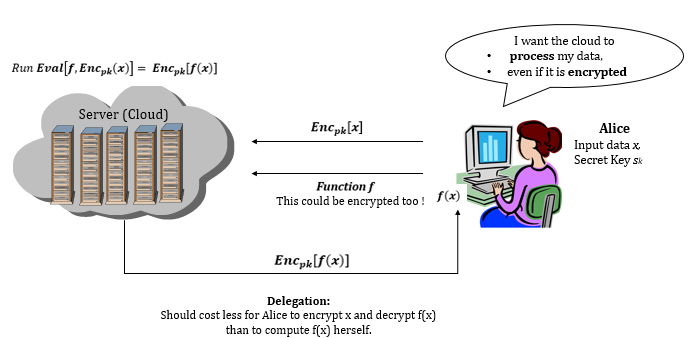
\includegraphics[width=\linewidth]{figures/fhew_prob_stmt.PNG}
 \caption{FHE: Problem Statement
 \cite{shai_he}}
 \label{fig:fhew_prob_stmt}
\end{figure}
\subsection{Background}
\label{4_1_1}
\subsubsection*{Homomorphism}
Given two groups, G and H, Homomorphism from G to H can be defined as a function \textit{f: $G \rightarrow H$}, such that:
\begin{adjustwidth}{2cm}{}
f($g_1$ * $g_2$) = f($g_1$) * f($g_2$), \\
$g_1$, $g_2$ : Elements in \textit{G},\\
* : Operation in \textit{G}, \\
* : Operation in \textit{H}
\end{adjustwidth}
\subsubsection*{Steps in FHE}
Fully homomorphic encryption scheme $\epsilon$ has 4 key steps:\\
1. $KeyGen_\epsilon$($\lambda$)\\
It involves generation of random secret key, which is an odd integer \textit{p}, P-bits long. The security parameter $\lambda$ dictates the bit-length of the key.
\begin{itemize}
\item Symmetric Encryption: \\
Encryption and Decryption are performed using the same secret key.  
\item Asymmetric Encryption:\\ Encryption is done using a public key ($p_k$) and Decryption using a secret key ($s_k$).
\end{itemize}
2. $Encrypt_\epsilon$(\textit{p,m})\\
Given the security parameter $\lambda$, 
\begin{adjustwidth}{2cm}{}
N = $\lambda$; P = $\lambda^2$; Q = $\lambda^5$
\end{adjustwidth}
\underline{Scheme \cite{gentry2010computing}:}\\
To encrypt a bit \textit{m} $\in$ \{0,1\}, set \textit{m'= m mod 2}, a random N-bit number.
\begin{adjustwidth}{2cm}{}
Output ciphertext: \textit{c $\leftarrow$ m' + pq},
\end{adjustwidth}
where \textit{q} is a random Q-bit integer.
\begin{adjustwidth}{2cm}{}
i.e. \textit{c $\leftarrow$ m mod 2 + pq}
\end{adjustwidth}
3. $Decrypt_\epsilon$(\textit{p,c})
\begin{adjustwidth}{2cm}{}
Output: \textit{c' mod 2}, 
\end{adjustwidth}where \textit{c' = c mod p} is an integer in the range \textit{(-p/2, p/2)} and \textit{p} divides \textit{c-c'}.\\
\textit{c - c' = c - c mod p = c (1 - mod p)} is divisible by \textit{p}. Hence, the ciphertexts of $\epsilon$ are near-multiples of \textit{p}.\\
To maintain a constant complexity for decryption, any two ciphertexts $c_1$ and $c_2$ outputted from the encryption scheme should be of the same size \cite{gentry2010computing}. Size of the ciphertext and the time taken to decrypt should be independent of the complexity of function \textit{f}, delegated to the cloud.\newline\newline
4. $Evaluate_\epsilon$(\textit{$p_k$, f, $c_1$, $c_2$, ... $c_t$})\\For any function \textit{f} in a set of permissible functions \textit{$F_\epsilon$}, and ciphertexts \textit{$c_1$, $c_2$... $c_t$}, where \textit{$c_i$} $\leftarrow$ \textit{$Encrypt_\epsilon$}(\textit{$p_k$, $m_i$}), the following 2 steps are performed:
\begin{adjustwidth}{2cm}{}
\textit{c} $\leftarrow$ \textit{$Encrypt_\epsilon$[ f ($c_1$, $c_2$, ... $c_t$)]}\\
$Decrypt_\epsilon$(c , $s_k$) = \textit{f ($m_1$, $m_2$, ... $m_t$)}
\end{adjustwidth}
\begin{figure}[h!]
 \centering
 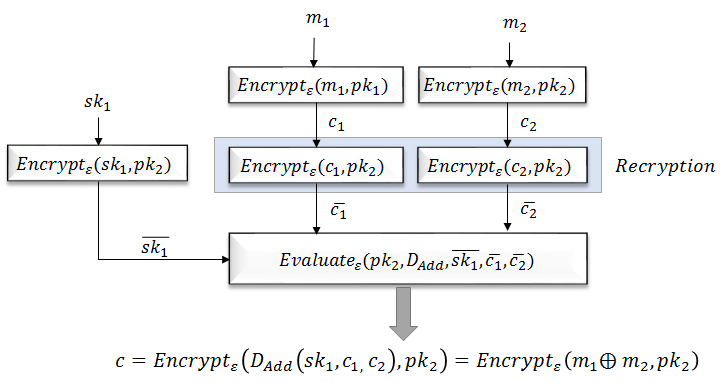
\includegraphics[width=\linewidth]{figures/Eval_FHE.png}
 \caption{Homomorphic Encryption Scheme : Example
 \cite{gentry2010computing}}
 \label{fig:Eval_FHE}
\end{figure}
This scheme guarantees one-wayness and semantic security against chosen plain-text attacks, as it is probabilistic \cite{gentry2010computing}. Figure \ref{fig:Eval_FHE} shows 2 messages $m_1$ and $m_2$ encrypted using public key $pk_1$ whose associated secret key is $sk_1$. $Evaluate_\epsilon$ takes in the resultant ciphertexts $c_1$, $c_2$ and secret key $sk_1$ encrypted under another key $pk_2$ and outputs \textit{c} which is an encryption of $D_\epsilon$ result under $pk_2$.
\subsubsection*{Concept of Bootstrapping}
\begin{figure}[h!]
 \centering
 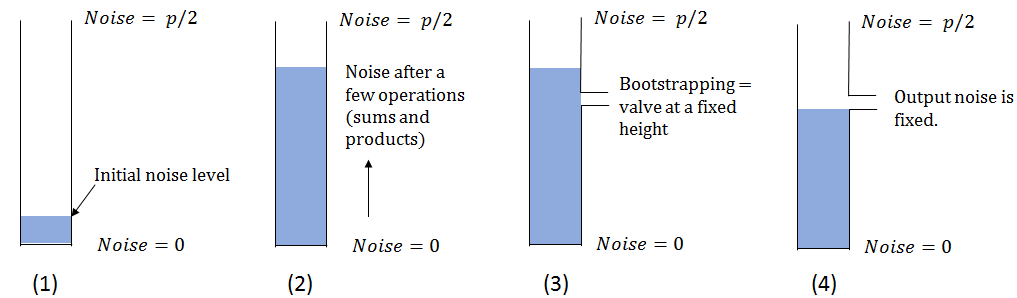
\includegraphics[width=\linewidth]{figures/bootstrapping.png}
 \caption{Homomorphic Decryption: Example
 \cite{he_utoronto}}
 \label{fig:bootstrapping}
\end{figure}
Decryption reduces the noise. However, decrypting the data in remote server can compromise security. So, homomorphic decryption described in Figure \ref{fig:Eval_FHE} is used to reduce the noise level, so that the result is decipherable at the receiver. 
\subsection{Existing code flow}
\label{4_1_1}
\begin{figure}[h!]
 \centering
 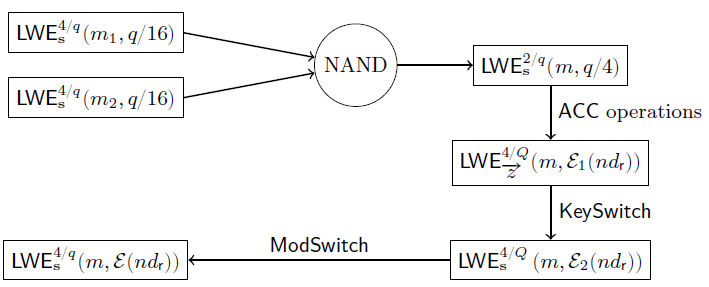
\includegraphics[width=0.8\linewidth]{figures/FHEW.PNG}
 \caption{Cycle of simple NAND operation
 \cite{ducas2015fhew}}
 \label{fig:FHEW}
\end{figure}
The FHEW Library \cite{fhew_lib} uses the ring lattice for encryption and bootstrapping, to reduce the computation time to quasi-linear complexity (Using FFT) as opposed to the quadratic complexity of previous methods \cite{ducas2015fhew}.\newline\newline
The \textit{Learning With Errors} (LWE) encryption scheme has been used to generate ciphertexts, with a message modulus of 4 and error bound of q/16. The specifics of this scheme have been described in great detail in \cite{ducas2015fhew} for further reading, and shall not be covered in this thesis. A random evaluation key, constituting a bootstrapping key and switching key is generated for a given LWE secret key. Both encryption and recryption (Figure \ref{fig:Eval_FHE}) use the LWE scheme but with different keys. Two ciphertexts LWE-encrypted using a n-dimensional secret key (n = 500) are fed to the Homomorphic NAND block:\newline \newline
HomNAND: $LWE_{s}^\frac{4}{q}$($m_0$, q/16) x $LWE_{s}^\frac{4}{q}$($m_1$, q/16)$\rightarrow$ $LWE_{s}^\frac{2}{q}$($m_0 \bar{\wedge} m_1$, q/4)\newline \newline
where LHS denotes ciphertext inputs encrypting binary messages, $m_0, m_1$ $\in$ \{0,1\} with error limit as q/16. RHS is the HomNAND output which is an encryption of the logical NAND of the two input messages = 1 - $m_0.m_1$ = $m_0 \bar{\wedge} m_1$, with an error bound of q/4.
The switching key facilitates conversion of LWE encryption with one secret key to another LWE encryption using a different secret key. Modulus switching helps switch the LWE ciphertexts from one modulus (Q) to another (q). \\The most efficient Bootstrapping method proposed by the author is the one using FFTs (Section 5.3, \cite{ducas2015fhew}). The Fastest Fourier Transform in the West (FFTW) Library \cite{FFTW05} is an open-source benchmark library for optimized software FFT computations. This library has been used for performing FFTs and inverse FFTs in the FHE algorithm, with double-precision floating point accuracy. 
\subsection{Hot-Spots for Hardware Acceleration}
\label{4_1_2}
One major difference in FPGA programming, be it RTL or HLS, is the bit-width precision. Register sizes are deterministic at compile time. Libraries such as $<ap\_cint.h>$ and $<ap\_int.h>$ in Vivado HLS facilitate specification of bit-accurate variables.  We notice that FFTW Library required by FHEW library is compiled for double-precision floating point accuracy which is 64-bits long by default. Usually, Embedded devices are memory and power constrained. Hence, exploring the accuracy of results with varying bit-widths is another interesting aspect to investigate, for a holistic analysis of hardware acceleration using FPGAs.\\
Software Profiling results have confirmed that the Homomorphic NAND operation takes up the maximum execution time. Each HomNAND operation makes several calls to Accumulator as illustrated in Table \ref{table:sw_hotspots_fhe}. The accumulator in turn calls the 2048-point FFT and IFFT routines several times.
\begin{table}[htbp]
\caption{Analysis of Software Bottlenecks}
\centering
\begin{tabular}{c p{4.5cm} c}
\toprule
HomNAND Test Count & Function & Number of function calls\\
\midrule
\multirow{4}{*}{0}&FFT&396002\\
\cmidrule(r{4pt}){2-3}
  &Inverse FFT&132000\\
\cmidrule(r{4pt}){2-3}
 &Homomorphic NAND&0\\
\cmidrule(r{4pt}){2-3}
 &Add to Accumulator&0\\
\midrule
\multirow{4}{*}{1}&FFT&499430\\
\cmidrule(r{4pt}){2-3}
 &Inverse FFT&166470\\
\cmidrule(r{4pt}){2-3}
 &Homomorphic NAND&3\\
\cmidrule(r{4pt}){2-3}
 &Add to Accumulator&2872\\
\bottomrule
\end{tabular}
\label{table:sw_hotspots_fhe}
\end{table}
The tabulated values are averages obtained from 5 runs of the application in each of the two cases, HomNAND Test for 0 and 1 rounds. The number of function calls is not deterministic but usually around a certain range, due to the random nature of input, secret and bootstrapping keys. Each HomNAND Test involves 3 HomNAND function calls in the implemented FHE design \cite{fhew_lib} \ref{table:sw_hotspots_fhe}. This is because the circuit under test is defined by: (\textbf{a} NAND \textbf{b}) NAND (\textbf{c} NAND \textbf{d}).
\subsubsection{Dimensionality Analysis}
\begin{table}[]
\centering
\caption{Dimensionality Analysis (Section 6.2, \cite{ducas2015fhew})}
\label{tab:fhew_dim}
\begin{tabular}{@{}m{0.5\linewidth} m{0.5\linewidth}@{}}
\toprule
\multicolumn{1}{c}{\textbf{Parameter}} & \multicolumn{1}{c}{\textbf{Size}} \\ \midrule
\multicolumn{1}{l}{LWE Secret Key} & \multicolumn{1}{l}{Array of size 500} \\ \midrule
\multicolumn{1}{l}{\multirow{2}{*}{Evaluation Key}} & \multicolumn{1}{l}{BootstrappingKey{[}500{]}{[}23{]}{[}2{]}} $\approx$ 1032 MBytes \\ \cmidrule(l){2-2} 
\multicolumn{1}{l}{} & \multicolumn{1}{l}{SwitchingKey{[}1024{]}{[}25{]}{[}7{]} $\approx$ 314 MBytes} \\ \midrule
\multicolumn{1}{l}{HomNAND Inputs} & \multicolumn{1}{l}{1-bit} \\ \midrule
\multicolumn{1}{c}{\multirow{2}{*}{\begin{tabular}[c]{@{}c@{}}HomNAND Output Cipher\\ (a,b);\end{tabular}}} & \multicolumn{1}{l}{\begin{tabular}[c]{@{}l@{}}a{[}500{]} - coefficient vector over a \\ cyclotomic ring R in Z{[}X{]}/$X^N$+1;\end{tabular}} \\ \cmidrule(l){2-2} 
\multicolumn{1}{c}{} & \multicolumn{1}{l}{b = \textbf{a.s} + e, where e is the error.} \\ \midrule
\multicolumn{1}{l}{Decrypt Output} & \multicolumn{1}{l}{32 bits} \\ \bottomrule
\end{tabular}
\end{table}
Table \ref{tab:fhew_dim} shows the dimensions of the inputs, intermediate values, secret keys and output in the encryption scheme. The bootstrapping and switching keys used in AddToAccumulator block of HomNAND operation are of huge sizes and hence, replicating multiple AddToAccumulator blocks in the hardware could be costly, without prior optimizations. Table \ref{table:sw_hotspots_fhe} shows that each Homomorphic NAND test involves around $\frac{499430 - 396002}{3}$ = 34476 FFT operations and the author confirms in Section 6.2, \cite{ducas2015fhew} that as high as 48000 FFTs are performed per NAND gate. 
\begin{table}[htbp]
\caption{Software Computation Time}
\centering
\begin{tabular}{l c}
\toprule
\textbf{Operation} & \textbf{Computation Time ($\mu$s)}\\
\midrule
FFTW FFT &30.892\\
\midrule
FFTW IFFT &23.93\\
\bottomrule
\end{tabular}
\label{table:fft_time}
\end{table}
The Table \ref{table:fft_time} illustrates the average execution time of a single FFT and IFFT, taken across 500 readings in a quad-core CPU. Since the speed of the algorithm depends on the speed of FFTs, porting this portion to hardware helps achieve a faster execution. We observe that FFTW is highly efficient in terms of runtime in software. However, it is a huge library and not hardware-friendly. \newline \newline
\subsection{Results}
\label{4_1_2}
\subsubsection*{Precision Analysis}
To determine whether double-precision floating point FFT is required to preserve the functionality of FHEW, the source code of FHEW was linked to different precision libraries and output analyzed. The configure script that comes with the library source files is used to generate Makefile. By using different compiler flags \cite{fftw_unix}, the FFTW library can be compiled for:
\begin{itemize}
\item single precision floating point
\begin{scriptsize}
\linuxbash
\begin{lstlisting}
$ sudo ./configure --enable-float
\end{lstlisting}
\end{scriptsize}
\item quadruple-precision floating point (\_\_float128)
\begin{scriptsize}
\linuxbash
\begin{lstlisting}
$ sudo apt-get install libquadmath
$ sudo ./configure --enable-quad-precision
\end{lstlisting}
\end{scriptsize}
\item long double 
\begin{scriptsize}
\linuxbash
\begin{lstlisting}
$ sudo ./configure --enable-long-double
\end{lstlisting}
\end{scriptsize}
\end{itemize}
When no option is specified, the default precision is \textit{double}. The below commands install the library with the new precision settings.
\begin{scriptsize}
\linuxbash
\begin{lstlisting}
$ make
$ make install
\end{lstlisting}
\end{scriptsize}
The source code of FHEW is linked to the new libraries: \textbf{-lfftw3f} (for float) or \textbf{-lfftw3l} (for long double) or \textbf{-lfftw3q -lquadmath -lm} (for quad-float) instead of the default library \textbf{-lfftw3}.\newline\newline
All lower-case instances of "fftw\_" in the FFT function calls and datatypes are replaced by fftwf\_ (for float) or fftl\_ (for long double) or fftwq\_ (for quad-float).\\
\textbf{Example:} The datatype \textbf{fftw\_complex} becomes \textbf{fftwf\_complex} or \textbf{fftwl\_complex} or \textbf{fftwq\_complex }depending on the desired precision.\newline \newline
As our intention is reduction of bit-width, the experiments were based on single-precision and quad-precision float. Upon making the above-mentioned changes, the FHEW functionality was not preserved due to reduction in accuracy. Supporting the analysis, the authors of \cite{ducas2015fhew} have stated that double-precision float is barely sufficient to contain the error levels within an acceptable range (Section 6.3, \cite{ducas2015fhew}). Figure \ref{fig:fft_precision_loss} illustrates the loss of functionality upon linking the source code to a lower precision FFT.
\begin{figure}[h!]
 \centering
 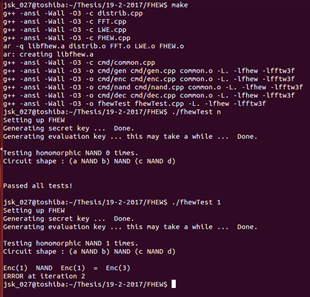
\includegraphics[width=0.5\linewidth]{figures/fft_precision_loss.png}
 \caption{Precision Loss with single-precision float}
 \label{fig:fft_precision_loss}
\end{figure}
From the above experiments, we conclude that of the standard datatypes, \textbf{double} is the lowest allowable precision that preserves the homomorphic encryption functionality. \newline\newline
FFTs can also be performed in integer domain using Number Theoretic Transform library (NTL) used in \cite{helib}. NTL involves convolution of 2 sequences modulo a prime number. Hence, the choice of modulus with respect to sequence length is restricted \cite{bhattacharya2004some}. FFTW has proved to be much more optimized and faster than the latter as stated in Section 6.3, \cite{ducas2015fhew}, which is why FHEW is an improvement over HELib \cite{shai_he} which uses NTL, in terms of Bootstrapping runtime. As the optimization objective is to improve run-time, FFT function can be hand-optimized for hardware acceleration and the functional correctness verified, by integrating with the existing software implementation.
\subsubsection*{FFT Offload}
Various FFT implementations were explored, intuitively optimized and their runtime performance was studied using High-level synthesis tools.
Firstly, the Xilinx FFT IP Core \cite{logicore2012fast} was analyzed and its usage studied. It implements the Cooley Tukey (Radix-4 DIT) FFT and accepts input in full-precision fixed point, scaled fixed point and block floating point . Since double-precision inputs are not supported by this hard block, it is not an ideal candidate for our application's acceleration. Then, a Cooley Tukey FFT algorithm was implemented, of size N given by the product $N_1$.$N_2$ where $N_1$ naive DFTs, each of size $N_2$ were performed. 
\begin{table}[htbp]
\centering
\caption{Execution time of unoptimized Cooley Tukey implementation with transform length N = 1024 in Avnet Zedboard Evaluation Platform}
\label{tab:ct_fft_1}
\begin{tabular}{|c|l|l|l|l|l|}
\hline
\textbf{N1} & 512 & 256 & 128 & 64 & 32 \\ \hline
\textbf{N2} & 2 & 4 & 8 & 16 & 32 \\ \hline
\textbf{Execution Time (s)} & 1.5 & 0.77 & 0.38 & 0.23 & 0.18 \\ \hline
\end{tabular}
\end{table}
From Table \ref{tab:ct_fft_1}, we see that the execution time was in the order of seconds, irrespective of the values of $N_1$ and $N_2$. Thus, this implementation was further improved by doing loop and function optimizations, integrated to the FHEW code and the functional correctness was verified. Taking it further, a radix-2 butterfly DIF FFT logic was implemented. \newline \newline For these implementations to be synthesizable by the high-level synthesis tool, recursive calls and dynamic memory allocation were avoided and all pointers were made deterministic at compile time. Various optimization directives were intuitively chosen to offer improved runtime performance and the best optimization was identified. The pros and cons of all three implementations were studied to decide on which best suits our need.  
\subsubsection{Hand-optimized non-recursive 1-D FFT}
Table \ref{tab: dse_1dfft} illustrates the clock period, latency and utilization estimates upon applying different optimization directives to the hand-optimized FFT implementation for hardware. We observe that solution 4 offers the most optimal area-latency design point. 
\newcolumntype{L}{>{\centering\arraybackslash}p{{0.15\linewidth}}}
\begin{table}[htbp]
\centering
\caption{Design Space Exploration for non-recursive 1-D FFT}
\label{tab: dse_1dfft}
\begin{tabular}{|m{2cm}|m{1.5cm}|L|L|L|L|L|}
\hline
\multicolumn{7}{|c|}{\textbf{Target: Avnet Zedboard Evaluation xc7z020clg484-1}} \\ \hline
\multicolumn{2}{|l|}{} & \textbf{Solution 1} & \textbf{Solution 2} & \textbf{Solution 3} & \textbf{Solution 4} & \textbf{Solution 5} \\ \hline
\multicolumn{2}{|c|}{\textbf{Optimization}} & No directives. & Loop 0: Pipeline& Loop 0: Unroll & Loop 0 \& 2: Pipeline & Loop 0: Pipeline, Loop 2: Unroll \\ \hline
\multicolumn{2}{|c|}{\textbf{\begin{tabular}[c]{@{}c@{}}Estimated\\Clock Period\\(ns)\end{tabular}}} & 9.83 & 9.83 & 12.93 & 11.96 & 12.19 \\ \hline
\multirow{2}{*}{\textbf{\begin{tabular}[c]{@{}c@{}}Latency\\ (cycles)\end{tabular}}} & \textbf{Min} & 295730178 & 295705626 & 297810991 & 5387290 & 8048665 \\ \cline{2-7} 
 & \textbf{Max} & 945847298 & 945822746 & 947928111 & 5387290 & 12492825 \\ \hline
\multirow{4}{*}{\textbf{\begin{tabular}[c]{@{}c@{}}Utilization\\ Estimates\end{tabular}}} & \textbf{BRAM} & 13 & 13 & 13 & 8 & 13234 \\ \cline{2-7} 
 & \textbf{DSP48E} & 67 & 73 & 234 & 105 & 31410 \\ \cline{2-7} 
 & \textbf{FF} & 7235 & 8245 & 149093 & 32308 & 4632256 \\ \cline{2-7} 
 & \textbf{LUT} & 24133 & 26896 & 117748 & 70551 & 19331620 \\ \hline
\end{tabular}
\end{table}

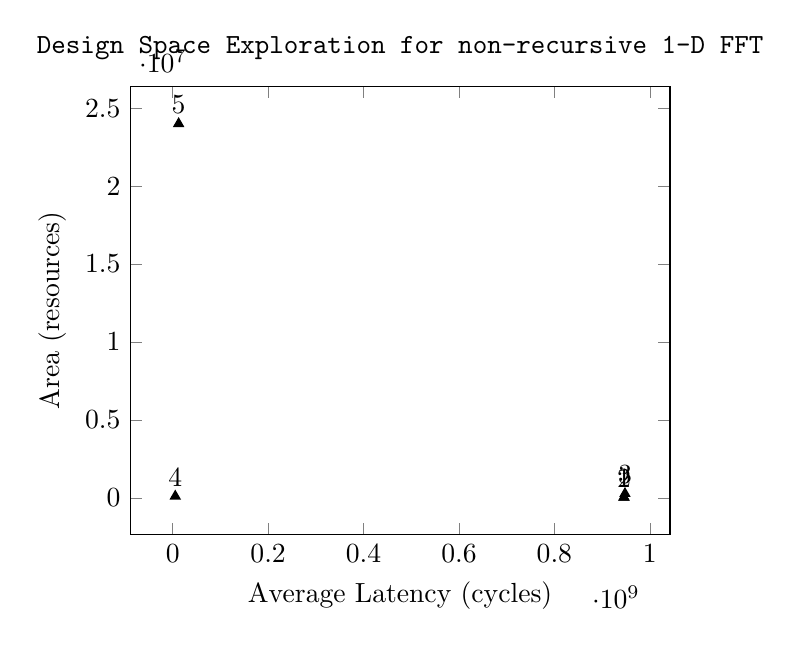
\begin{tikzpicture}
\label{graph:dse_1dfft}
\centering
	\begin{axis}[
		xlabel= Average Latency (cycles),
		ylabel=Area (resources),     
        nodes near coords, % Place nodes near each coordinate
    point meta=explicit symbolic, % The meta data used in the nodes is not explicitly provided and not numeric
	    title={\texttt{Design Space Exploration for non-recursive 1-D FFT}}]        
	\addplot[mark=triangle*, only marks, mark options={fill=black}] 
    table [% Provide data as a table
     meta index=2 % the meta data is found in the third column
     ] {
   x          y     label
945847298    31448    1
945822746    35227    2
947928111   267088    3
5387290     102972    4
12492825  24008520    5
	};
	\end{axis}
\end{tikzpicture}

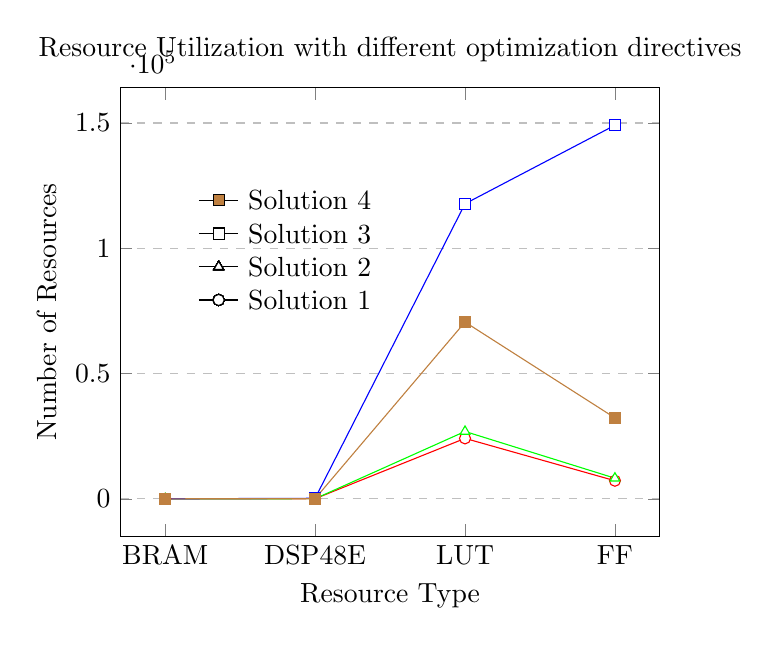
\begin{tikzpicture}
\begin{axis}[
    title={Resource Utilization with different optimization directives},
    xlabel={Resource Type},
    ylabel={Number of Resources},
    xtick=data,    
    legend pos=north west,
    ymajorgrids=true,
    grid style=dashed, 
    symbolic x coords={BRAM, DSP48E, LUT, FF},
]
 
\addplot[
    mark=*, mark options={fill=white}, color = red
    ]
    coordinates {
    (BRAM,13)
    (DSP48E,67)
    (LUT,24133)
    (FF,7235)
    };   

\addplot[
    mark=triangle*, mark options={fill=white}, color = green
    ]
    coordinates {
    (BRAM,13)
    (DSP48E,73)
    (LUT,26896)
    (FF,8245)
    };    
    
\addplot[
    mark=square*, mark options={fill=white}, color = blue
    ]
    coordinates {
    (BRAM,13)
    (DSP48E,234)
    (LUT,117748)
    (FF,149093)
    };    
    
\addplot[
    mark=square*, mark options={fill=brown}, color = brown
    ]
    coordinates {
    (BRAM,8)
    (DSP48E,105)
    (LUT,70551)
    (FF,32308)
    };    
\end{axis}    
    \begin{scope}[shift={(1,3)}] 
	\draw (0,0) -- 
		plot[mark=*, mark options={fill=white}, color=red] (0.25,0) -- (0.5,0) 
		node[right]{Solution 1};
	\draw[yshift=\baselineskip] (0,0) -- 
		plot[mark=triangle*, mark options={fill=white}, color=green] (0.25,0) -- (0.5,0)
		node[right]{Solution 2};
	\draw[yshift=2\baselineskip] (0,0) -- 
		plot[mark=square*, mark options={fill=white}, color=blue] (0.25,0) -- (0.5,0)
		node[right]{Solution 3};
	\draw[yshift=3\baselineskip] (0,0) -- 
		plot[mark=square*, mark options={fill=brown}, color = brown] (0.25,0) -- (0.5,0)
		node[right]{Solution 4};
	\end{scope}

\end{tikzpicture}

\subsubsection{Cooley Tuckey Radix-2 DIF FFT}
DIF FFT takes inputs in bit-reversed order and produces outputs in natural order. Shift operators are used instead of the costly multipliers. This implementation is in-place to reduce migration costs and less intuitive, but better optimized for hardware. \newline\newline
Appendix \ref{fhewcode3:CTfft} shows that some loop bounds are not statically defined. So, the HLS tool cannot determine the number of iterations of a variable-length loop at runtime and hence, cannot supply the latency estimates. To circumvent this problem, the directive "Loop Trip Count" is applied by manually specifying the maximum number of times this loop will be executed, at compile time.\newline\newline

\begin{table}[htbp]
\centering
\caption{Design Space Exploration for Cooley Tukey Radix-2 DIF FFT}
\label{tab:dse_ctfft}
\begin{tabular}{|m{2cm}|m{1.5cm}|L|L|L|L|}
\hline
\multicolumn{6}{|c|}{\textbf{Target: Avnet Zedboard Evaluation xc7z020clg484-1}} \\ \hline
\multicolumn{2}{|l|}{} & \textbf{Solution 1} & \textbf{Solution 2} & \textbf{Solution 3} & \textbf{Solution 4} \\ \hline
\multicolumn{2}{|c|}{\textbf{Optimization}} & \begin{tabular}[c]{@{}c@{}}Loops 1,2:\\Trip\\Count \\= 512\end{tabular} & \begin{tabular}[c]{@{}c@{}}Loops 1,2:\\Trip\\Count \\= 512,\\Loop 3:\\Pipeline\end{tabular} & \begin{tabular}[c]{@{}c@{}}Loops 1,2:\\Trip\\Count \\= 512,\\ Loop 3:\\Unroll\end{tabular} & \begin{tabular}[c]{@{}c@{}}Loops 1,2:\\Trip\\Count \\= 512,\\ Loop 3:\\Unroll\\(factor 16)\end{tabular} \\ \hline
\multicolumn{2}{|c|}{\textbf{Estimated Clock Period}} & 8.23 & 8.23 & 8.23 & 8.23 \\ \hline
\multirow{2}{*}{\textbf{\begin{tabular}[c]{@{}c@{}}Latency\\ (cycles)\end{tabular}}} & \textbf{Min} & 2170 & 3195 & 1112 & 1210 \\ \cline{2-6} 
 & \textbf{Max} & 49871994 & 49871995 & 49869912 & 49871994 \\ \hline
\multirow{4}{*}{\textbf{\begin{tabular}[c]{@{}c@{}}Utilization\\ Estimates\end{tabular}}} & \textbf{BRAM\_18K} & 0 & 0 & 0 & 0 \\ \cline{2-6} 
 & \textbf{DSP48E} & 56 & 56 & 56 & 56 \\ \cline{2-6} 
 & \textbf{FF} & 4511 & 4513 & 131834 & 6996 \\ \cline{2-6} 
 & \textbf{LUT} & 8529 & 8529 & 67506 & 9932 \\ \hline
\end{tabular}
\end{table}

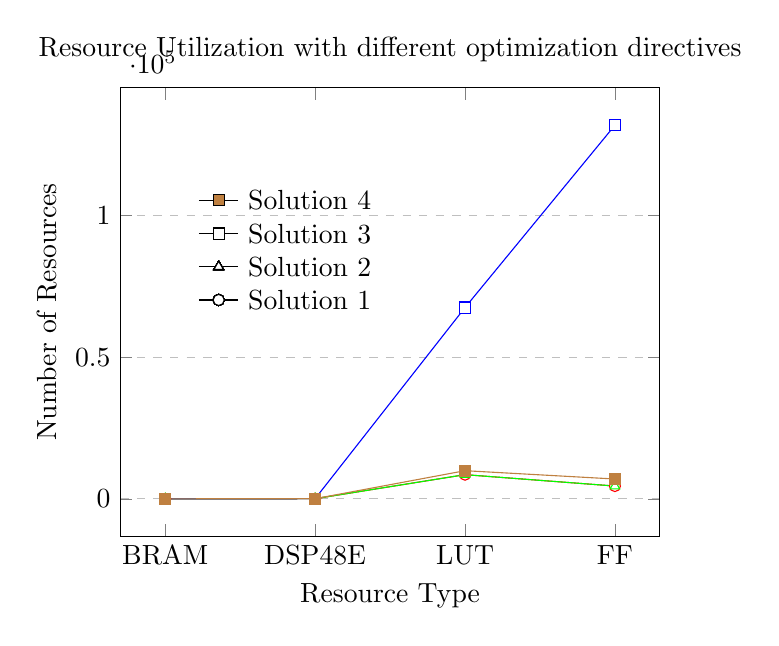
\begin{tikzpicture}
\begin{axis}[
    title={Resource Utilization with different optimization directives},
    xlabel={Resource Type},
    ylabel={Number of Resources},
    xtick=data,    
    legend pos=north west,
    ymajorgrids=true,
    grid style=dashed, 
    symbolic x coords={BRAM, DSP48E, LUT, FF},
]
 
\addplot[
    mark=*, mark options={fill=white}, color = red
    ]
    coordinates {
    (BRAM,0)
    (DSP48E,56)
    (LUT,8529)
    (FF,4511)
    };   

\addplot[
    mark=triangle*, mark options={fill=white}, color = green
    ]
    coordinates {
    (BRAM,0)
    (DSP48E,56)
    (LUT,8529)
    (FF,4513)
    };    
    
\addplot[
    mark=square*, mark options={fill=white}, color = blue
    ]
    coordinates {
    (BRAM,0)
    (DSP48E,56)
    (LUT,67506)
    (FF,131834)
    };    
    
\addplot[
    mark=square*, mark options={fill=brown}, color = brown
    ]
    coordinates {
    (BRAM,0)
    (DSP48E,56)
    (LUT,9932)
    (FF,6996)
    };    
\end{axis}    
    \begin{scope}[shift={(1,3)}] 
	\draw (0,0) -- 
		plot[mark=*, mark options={fill=white}, color=red] (0.25,0) -- (0.5,0) 
		node[right]{Solution 1};
	\draw[yshift=\baselineskip] (0,0) -- 
		plot[mark=triangle*, mark options={fill=white}, color=green] (0.25,0) -- (0.5,0)
		node[right]{Solution 2};
	\draw[yshift=2\baselineskip] (0,0) -- 
		plot[mark=square*, mark options={fill=white}, color=blue] (0.25,0) -- (0.5,0)
		node[right]{Solution 3};
	\draw[yshift=3\baselineskip] (0,0) -- 
		plot[mark=square*, mark options={fill=brown}, color = brown] (0.25,0) -- (0.5,0)
		node[right]{Solution 4};
	\end{scope}

\end{tikzpicture}

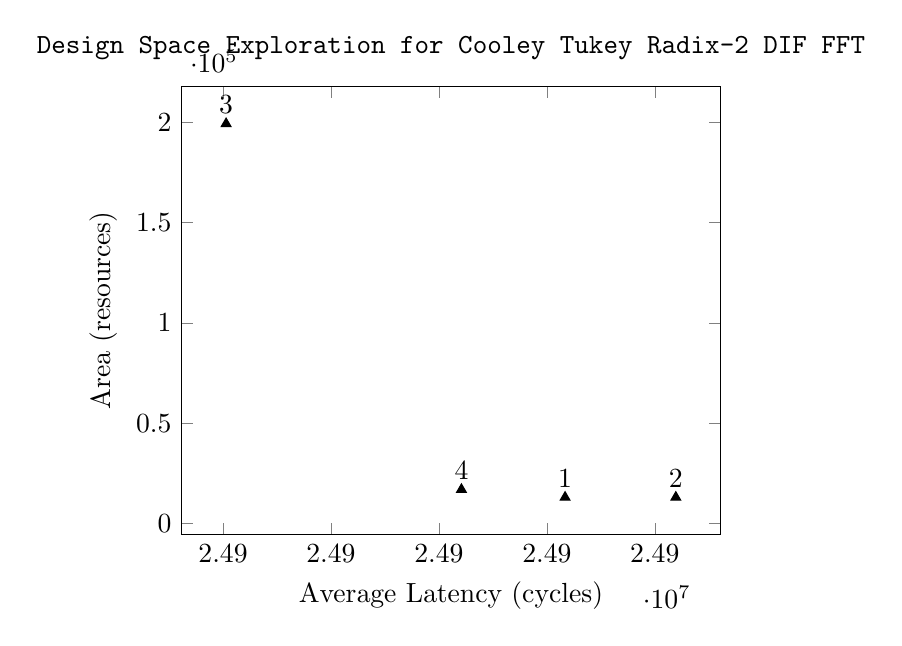
\begin{tikzpicture}
\label{graph:dse_CTfft}
\centering
	\begin{axis}[
		xlabel=Average Latency (cycles),
		ylabel=Area (resources),     
        nodes near coords, % Place nodes near each coordinate
    point meta=explicit symbolic, % The meta data used in the nodes is not explicitly provided and not numeric
	    title={\texttt{Design Space Exploration for Cooley Tukey Radix-2 DIF FFT}}]        
	\addplot[mark=triangle*, only marks, mark options={fill=black}] 
    table [% Provide data as a table
     meta index=2 % the meta data is found in the third column
     ] {
   x          y     label
24937082	13096    1
24937595	13098    2
24935512	199396   3
24936602	16984    4
	};
	\end{axis}
\end{tikzpicture}
\newline From the plot \ref{graph:dse_CTfft}, we see that solution 3 gives the best case latency. However, there are not enough LUTs in the target board to implement this design. Hence, optimizations of solution 4 are more appropriate for a practical best-case latency scenario. 
\newcolumntype{C}{>{\centering\arraybackslash}p{{0.25\linewidth}}}
\subsubsection{MachSuite FFT}
MachSuite is a collection of 19 diverse application benchmarks, which are high-level synthesizable. FFT algorithm which is one of the benchmark applications is explored to decide whether it meets our requirement.
\begin{table}[htbp]
\centering
\caption{Design Space Exploration for Machsuite FFT}
\label{tab:dse_machsuite}
\begin{tabular}{|m{2cm}|m{1.5cm}|m{3cm}|m{3cm}|}
\hline
\multicolumn{4}{|c|}{\textbf{Target: Avnet Zedboard Evaluation xc7z020clg484-1}} \\ \hline
\multicolumn{2}{|c|}{} & \textbf{Solution 1} & \textbf{Solution 2}\\ 
\hline
\multicolumn{2}{|c|}{\textbf{Optimization}} & \begin{tabular}[c]{@{}c@{}}Loop 0: Trip\\Count = 10,\\Loop 1: Trip\\Count = 1024\end{tabular} & \begin{tabular}[c]{@{}c@{}}Loops 1,2:\\Trip Count=512,\\Loop 3:\\Pipeline\end{tabular} \\ \hline
\multicolumn{2}{|c|}{\textbf{Estimated Clock Period}} & \makecell[c]{8.23} & \makecell[c]{8.23} \\ \hline
\multirow{2}{*}{\textbf{\begin{tabular}[c]{@{}c@{}}Latency\\ (cycles)\end{tabular}}} & \textbf{Min} & \makecell[c]{2170} & \makecell[c]{3195} \\ \cline{2-4} 
 & \textbf{Max} & \makecell[c]{49871994} & \makecell[c]{49871995} \\ \hline
\multirow{4}{*}{\textbf{\begin{tabular}[c]{@{}c@{}}Utilization\\ Estimates\end{tabular}}} & \textbf{BRAM\_18K} & \makecell[c]{0} & \makecell[c]{0} \\ \cline{2-4} 
 & \textbf{DSP48E} & \makecell[c]{56} & \makecell[c]{56} \\ \cline{2-4} 
 & \textbf{FF} & \makecell[c]{4511} & \makecell[c]{4513} \\ \cline{2-4} 
 & \textbf{LUT} & \makecell[c]{8529} & \makecell[c]{8529} \\ \hline
\end{tabular}
\end{table}

\subsubsection{Comparison of Execution Times}
\begin{table}[htbp]
\centering
\caption{Estimates of execution time in different FFT algorithms}
\label{tab:compare_fft}
\begin{tabular}{|m{0.2\linewidth}|m{0.25\linewidth}|m{0.25\linewidth}|m{0.25\linewidth}|}
\hline
 & \textbf{\makecell[c]{Non-recursive\\1-D FFT}} & \textbf{\makecell[c]{Radix-2\\DIF FFT}} &\textbf{MachSuite FFT}\\ \hline
\textbf{Best-case Execution Time} & 5387290 x 11.96 ns = 0.064 s & 1210 x 8.23 ns = 9.95 $\mu$s & 2170 X 8.23 ns = 17 $\mu$s \\ \hline
\end{tabular}
\end{table}

The execution time in Table \ref{tab:compare_fft} is calculated as the product of number of cycles and clock period. In Non-recursive 1-D FFT, execution time is of the order of a few milliseconds. As our application demands speed in the range of microseconds for gain over software implementation, Radix-2 FFT proves to be the optimal choice. \newline
\begin{adjustwidth}{2cm}{}
The ratio $R_{acceleration}$ = $\frac{t_{sw}}{t_{hw}}$ = $\frac{30.892}{9.95}$ = 3.1047\newline 
\end{adjustwidth} 
High-speed Streaming DMA Transfers from high performance ports of Zynq Processing system to Programmable logic via AXI Interface assure that the communication overhead is less. By using higher FPGA generations such as Virtex 7, a much higher speedup can be obtained and unroll factor increased. 